\documentclass{report}
\usepackage
[
        a4paper,% other options: a3paper, a5paper, etc
        left=2.5cm,
        right=2.5cm,
        % top=3cm,
        bottom=3cm,
        % use vmargin=2cm to make vertical margins equal to 2cm.
        % us  hmargin=3cm to make horizontal margins equal to 3cm.
        % use margin=3cm to make all margins  equal to 3cm.
]
{geometry}

% OPTIONS
% Versione estesa
% \def\extendedPdf

% \documentclass[a4paper,11pt]{report}
% Standard margins for SLU is 3.5 cm on each side. Add this code if desired:
% \usepackage[a4paper, left=3cm, right=3cm]{geometry}
\usepackage{fancyhdr}

\usepackage[T1]{fontenc}
\usepackage[utf8]{inputenc}
\usepackage[english]{babel}	% Not found
\usepackage{graphicx}
\usepackage{booktabs}
\usepackage{comment}
\usepackage{float}  %force image posistion
%\usepackage{siunitx}	% Not found
%\usepackage{pdfpages}   %inseting pages from an externl pdf
%\usepackage{natbib}
\usepackage{titlesec, color}
\usepackage[pdftex,pdfpagelabels,bookmarks,hyperindex,hyperfigures,hidelinks]{hyperref}
%hidelinks per nascondere i riquadri rossi che si verrebbero a creare attorno ai link generati da hyperref
\usepackage[open,openlevel=1]{bookmark}
%\usepackage{multirow}
%\usepackage[Bjornstrup]{fncychap}
%Options: Sonny, Lenny, Glenn, Conny, Rejne, Bjarne, Bjornstrup
%\usepackage{changepage}                 % adjust margins for selected portions
%\usepackage{lipsum}
\usepackage{csvsimple}
%\usepackage{pdflscape}
%\usepackage[usenames,dvipsnames]{xcolor}
\usepackage{listings}

\usepackage{amsmath}
\usepackage{tikz}
\usepackage{epigraph}
\usepackage{lipsum}

\renewcommand\epigraphflush{flushleft}
\renewcommand\epigraphsize{\normalsize}
\setlength\epigraphwidth{0.7\textwidth}



% -----------------------------------------------
% ---- Comandi simone header pagina - titolo ----
% -----------------------------------------------
\newcommand{\docrevision}{\ddmmyyyydate\today}
\newcommand{\projectname}{Modbus Client}
\newcommand{\projectdescription}{Modbus Client Manual }

\newcommand{\revision}{\docrevision}
\newcommand{\version}{v2.38}
\renewcommand{\chaptermark}[1]{\markboth{#1}{#1}}   % Chapter name in alto a sx senza "Capitolo x " davanti

\pagestyle{fancy}
\fancyhf{}
% \lhead{\revision}
\lhead{\leftmark}       % Titolo del capitolo
\chead{\projectname}    % Nome del Progetto
\rhead{Federico Turco}
\cfoot{\thepage}
% -----------------------------------------------

%\usepackage[a-1b]{pdfx}
%\usepackage[pdfa,pdfpagelabels,bookmarks,hyperindex,hyperfigures]{hyperref}
%\usepackage[pdfa, colorlinks=true,linkcolor=black,anchorcolor=black,citecolor=black,filecolor=black,menucolor=black,runcolor=black,urlcolor=black]{hyperref}
%\usepackage[pdfa]{hyperref}
%\usepackage[pdfpagelabels]{hyperref}

%\usepackage[pdfa,pdfpagelabels,bookmarks,hyperindex,hyperfigures,hidelinks]{hyperref}

% wide page for side by side figures, tables, etc
\newlength{\offsetpage}
\setlength{\offsetpage}{1.5cm}
\newenvironment{widepage}{\begin{adjustwidth}{-\offsetpage}{-\offsetpage}%
    \addtolength{\textwidth}{2\offsetpage}}%
{\end{adjustwidth}}

%micro

%----Gestione capitoli
%-\part
%-\chapter
%-\section
%-\subsection
%-\subsubsection
%-\paragraph
%-\subparagraph

%-tableofcontents
%-listoffigures
%-listoftables
%-printindex

%-printbibliography

\def \citeOpen {(fonte: }
\def \citeClose {)}

% Dimesioni default immagini
\def \imageSizeFull{1}
\def \imageSizeRegisterSmall{0.7}
\def \imageSizeRegister{0.8}

\setlength\parindent{0pt}

% DEFINIZIONE-CHAPTER-STYLE
\definecolor{gray75}{gray}{0.75}
\newcommand{\hsp}{\hspace{20pt}}
\titleformat{\chapter}[hang]{\Huge\bfseries}{\thechapter\hsp\textcolor{gray75}{|}\hsp}{0pt}{\Huge\bfseries}

% INIZIO-DOCUMENTO
\begin{document}

% INSERIMENTO-FRONTESPIZIO
\begin{titlepage}

\DeclareFixedFont{\titlefont}{T1}{phv}{b}{}{38pt}

\makeatletter                       
\def\printauthor{
    {\large \@author}}              
\makeatother
\author{
  \href{https://fedeturco.github.io/}{Federico Turco} \\
  \href{mailto:\federico.turco97@gmail.com}{federico.turco97@gmail.com}
  }

\begin{titlepage}

  \vspace*{3cm}
  \noindent
  \titlefont\projectname\par
  \epigraph{\projectdescription}{\docrevision}
  \null\vfill
  
  \noindent
  \hfill
  
  \begin{minipage}{0.45\linewidth}    % Autore a sinistra
  \begin{flushright}
  \printauthor
  \end{flushright}
  \end{minipage}
  \begin{minipage}{0.02\linewidth}    % Barra al centro
  \rule{1pt}{50pt}
  \end{minipage}
  \begin{minipage}[c]{0.4\linewidth}  % Logo a destra
  \begin{flushleft}
  \vspace*{3mm}
  \begin{figure}[H]
  
\includegraphics[height=17mm]{../../Logo/Modbus_logo_2.png}
  \end{figure}
  \end{flushleft}
  \end{minipage}
  \begin{tikzpicture}[remember picture,overlay]
  \node[] at ([yshift=-190px,xshift=-130px]current page.north east)
  {
  
\includegraphics[height=55mm]{../../Logo/Modbus_logo_2.png}
  };
  \end{tikzpicture}
  \end{titlepage}
\end{titlepage}

% Pagina vuota dopo titlepage
\shipout\null

% INDICE
\pagenumbering{roman}
\tableofcontents
\cleardoublepage
\pagenumbering{arabic}

% INDICE DELLE FIGURE
% \listoffigures

% INDICE DELLE TABELLE
% \listoftables

% DOCUMENTO

\chapter{Homepage}

This client is fully compliant with Modbus specifications,
it allows to read and write registers through both Modbus RTU and TCP protocols.
The main window contains the basic information to configure
the protocol comunication.
A USB-485 converter is required to query RTU slaves.
Starting from version v2.38
the client implements the new standard Modbus Secure.

\begin{figure}[H]
\centering
\includegraphics[width=0.85\textwidth]{../Img/Modbus_Client_Home_00.PNG}
\caption[Homepage]{Homepage}
\end{figure}

To test the connection to an IP address use the ping button,
if the ping is successful the button colors green otherwise red.
When the connection to a slave is successful the "Running" cube is colored
green (in the case of RTU connections it is considered successful if it succeeds in 
open the selected COM port correctly).
The next part of the document will describe the various tabs and associated functions.

\newpage
\section{Modbus Secure}

Starting with version 2.38, support has been introduced for
the ModBus Secure standard, according to the specifications described 
in the document MB-TCP-Security-v21\_2018-07-24.
Flagging the checkmark "Modbus Secure" enables the "Secure" configuration 
as shown in the following image:

\begin{figure}[H]
\centering
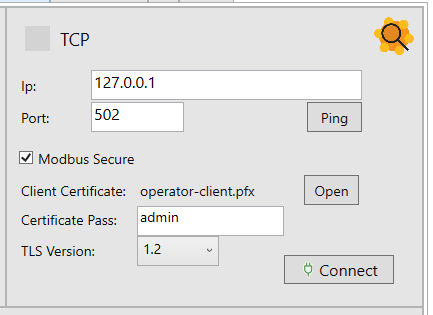
\includegraphics[width=0.6\textwidth]{../Img/ModBus_Home_Secure.PNG}
\caption[Modbus Secure]{Modbus Secure}
\end{figure}

The Modbus Secure protocol will be discussed in more detail later in section
\ref{secure}. It still works via TCP but standard datagrams are
encrypted through an SSL/TLS layer. When you check
the Modbus Secure box, a new field appears where you enter the port to be used
for secure connections, by default 802.
The Modbus Secure protocol requires (in addition to IP and port)
to load into the client
a password-protected certificate (password to be entered in the appropriate field).
The certificate should be uploaded in .pfx format, this
format contains, along with the certificate itself, also 
the private key to be used to encrypt the communication.
The client supports TLS v1.2 or 1.3 (the standard requires v1.2 or higher).


\chapter{Finestra principale}

Sulla destra della tab principale sono presenti 4 tab per leggere le varie risorse Modbus 
"FC 01 Coils", "FC02 Discrete Inputs", "FC 03 Holding Registers" e "FC04 Input Registers".

\section{FC01 - Coils}

La scheda Coils permette di leggere e scrivere uscite digitali con le funzioni FC01/FC05/FC15. I
pulsanti Read/Loop/Write vengono sbloccati solo se la connessione a un dispositivo è andata a
buon fine.

\begin{figure}[H]
\centering
\includegraphics[width=0.85\textwidth]{../Img/Modbus_Client_Coils_00.PNG}
\caption{FC01 - Coils}
\end{figure}

La funzione loop permette di leggere i registri indicati in polling, l'intervallo di interrogazione si
configura nella scheda impostazioni ("Settings"). 
Di default le celle lette vengono colorate di azzurro se il contenuto è popolato (inteso come $>$ 0).
In alto a destra sono presenti i comandi per leggere le risorse di un gruppo o tutte le risorse
di tipo coils configurate nel rpofilo corrente. La configurazione delle risorse così come la creazione e 
associazione dei gruppi viene descritto nel capitolo \ref{template}.

\newpage

Con il box "Read Coil Range" è possibile leggere un range di uscite digitali definito dall'utente,
sarà poi il programma eventualmente a dividere il comando in più richieste FC01 ciascuna di n coils
indicati sopra (nell'esempio seguente pari a 20). 
E' possibile inoltre forzare coils multiple (FC15) utilizzando il form in basso 
("Force Multiple Coils") o importando un file csv precedentemente esportato.

Le coils settate a 1 vengono colorate di verde se la scrittura va a
buon fine:

\begin{figure}[H]
\centering
\includegraphics[width=0.85\textwidth]{../Img/Modbus_Client_Coils_Write_00.PNG}
\caption{FC05 - Write Coils}
\end{figure}

Abilitando la modalità "Live Edit" è possibile modificare direttamente 
le coils editando la colonna "Value", in questo caso quando si modifica la riga il 
programma invia automaticamente il comando FC05 per impostare la coil al valore inserito.

\newpage
\section{FC02 - Discrete inputs}

La scheda Inputs permette di leggere ingressi digitali con le funzioni FC02. I pulsanti Read/Loop
come per la tab Coils vengono sbloccati solo se la connessione a un dispositivo è andata a buon
fine. I pulsanti "Read group" e "Read all" permettono di leggere registri precedentemente configurati 
nel template personalizzato (i registri vengono letti singolarmente sia che siano o meno consecutivi
tra di loro).

\begin{figure}[H]
\centering
\includegraphics[width=0.85\textwidth]{../Img/Modbus_Client_Inputs_00.PNG}
\caption{FC02 - Discrete Inputs}
\end{figure}

Con il box "Read Input Range" è possibile leggere un range di ingressi digitali definito dall'utente,
sarà poi il programma eventualmente a dividere il comando in più richieste FC02
ciascuna di n ingressi specificati nel box delle letture singole (nell'immagine sopra pari a 120).

\newpage
\section{FC03 - Holding registers}

La scheda Holding Registers permette di leggere e scrivere registri digitali a 16 bit con le funzioni
FC03/FC06/FC16.

\begin{figure}[H]
\centering
\includegraphics[width=0.85\textwidth]{../Img/Modbus_Client_HoldingReg_00.PNG}
\caption{FC03 - Holding Registers}
\end{figure}

Il valore del campo "Value" può essere visualizzato sia in decimale (DEC) che in esadecimale
(HEX). Nella tabella è possibile abilitare anche la visualizzazione del corrispondente valore in binario.
Ampliando la finestra è possibile visualizzare informazioni aggiuntive (che vengono configurate
nella finestra template), ad un registro holding infatti è possibile
associare un'etichetta per identificarne il contenuto o visualizzare il valore convertito in integer/
float/string/etc.. Utilizzare il menu a tendina view per configurare le colonne che si desidera visualizzare
nella tabella come mostrato nell'immagine seguente.

\begin{figure}[H]
\centering
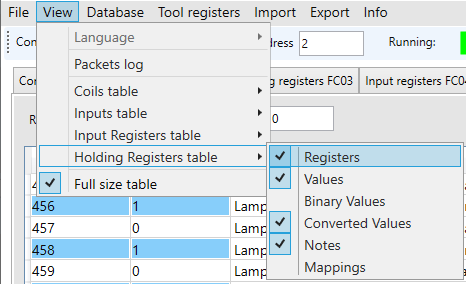
\includegraphics[width=0.40\textwidth]{../Img/Menu_View_Holding.PNG}
\caption{FC03 - View Tab Holding Registers}
\end{figure}

Con il box "Read Holding Register Range" è possibile leggere un range di registri definito
dall'utente (anche > 123), sarà poi il programma eventualmente a dividere il comando in più
richieste FC03 di n registri specificati nel box sopra (nell'immagine 120)
e a popolare la tabella con tutti i registri richiesti.

Spuntando il flag "Live Edit" è possibile inviare la scrittura dei registri automaticamente
modificando una cella delle colonne "Value", "Binary Value" o "Converted Value". La funzione
live risulta molto utile per modificare in diretta i registri visualizzati.

\begin{figure}[H]
\centering
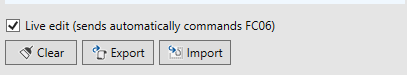
\includegraphics[width=0.40\textwidth]{../Img/ModBus_Client_HoldingReg_Live.PNG}
\caption{FC03 - Live edit}
\end{figure}

Le modifiche alle celle della colonna "Value" vengono inviate con la funzione FC06
(write single register), le modifiche alla colonna "Binary Value" vengono convertite da
binario e inviate sempre come FC06, mentre le modifiche alla colonna "Converted Value"
vengono inviate come FC06 o FC16 a seconda della tipologia del dato configurato (la funzione 
FC16 viene utilizzata
per variabili integer o float a 32 o 64 bit). Nella colonna value è possibile inserire 
valori in esadecimale, se la visualizzazione è già in esadecimale il valore inserito sarà considerato
sempre esadecimale, mentre nella visualizzazione decimale anteporre un "0x"/"x" o postporre un "h"
per indicare che il valore che si vuole inviare è scritto in esadecimale.

La tabella visualizzata può essere esportata in formato .csv o .json con il pulsante "Export" in basso
a destra. Tabelle esportate in csv possono essere importate e inviate allo slave con il pulsante "Import".
Questa funzione risulta comoda quando si vuole copiare una mappa di memoria da un PLC ad un altro o semplicemente
esportare un backup ripristinabile in qualsiasi momento.

\begin{figure}[H]
\centering
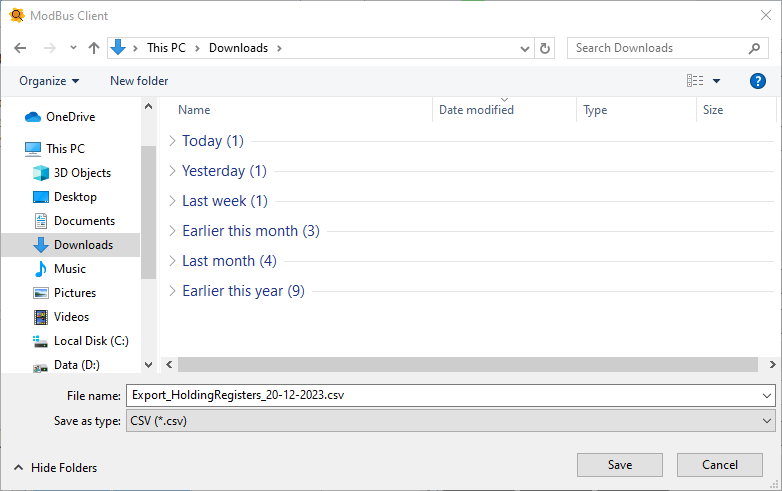
\includegraphics[width=0.70\textwidth]{../Img/ModBus_Client_HoldingReg_Import.PNG}
\caption{FC03 - Form import csv}
\end{figure}

\newpage
\section{FC04 - Input registers}

La scheda Input Registers permette di leggere registri a 16 bit con le funzioni FC04. I pulsanti
Read/Loop come per le altre tab vengono sbloccati solo se la connessione a un dispositivo è
andata a buon fine.

\begin{figure}[H]
\centering
\includegraphics[width=0.85\textwidth]{../Img/Modbus_Client_InputReg_00.PNG}
\caption{FC04 - Input Registers}
\end{figure}

Il valore del campo "Value" può essere visualizzato sia in decimale (DEC) che in esadecimale
(HEX). A fianco viene mostrato anche il valore in binario. Ampliando la finestra è possibile
visualizzare informazioni aggiuntive (che vengono configurate nella finestra template). Ad un
registro infatti è possibile associare un'etichetta per identificarne il contenuto o visualizzare il valore
convertito in integer/float/string/etc.. Per meglio chiarire questa parte si veda la sezione Template.
Con il box "Read Input Register Range" è possibile leggere un range di registri definito dall'utente
(anche > 123), sarà poi il programma eventualmente a dividere il comando in più richieste FC04 e
a popolare la tabella con tutti i registri richiesti.

\begin{figure}[H]
\centering
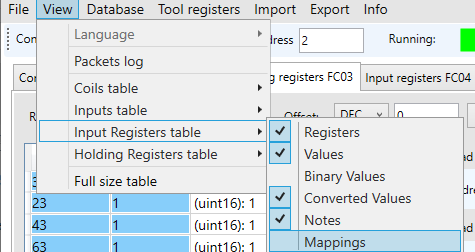
\includegraphics[width=0.60\textwidth]{../Img/Menu_View_InputReg.PNG}
\caption{FC04 - View TabInput Registers}
\end{figure}

Come per gli holding register è possibile selezionare dal menu view quali colonne mostrare nella tabella.

\newpage
\section{Diagnostica}

Nella tab diagnostica è possibile inviare comandi di diagnostica al dispositivo interrogato, 
si presti attenzione
che non tutti i dispositivi rispondono alla funzione FC08.

\begin{figure}[H]
\centering
\includegraphics[width=0.85\textwidth]{../Img/Modbus_Client_Diagnostic_00.PNG}
\caption{FC08 - Diagnostic}
\end{figure}

Funzioni FC08 supportate:

\begin{verbatim}
    - 00 Return Query Data
    - 01 Restart Comunications Option
    - 02 Return Diagnostic Register
    - 03 Change ASCII Input Delimeter
    - 04 Force Listen Only Mode
    - 10 Clear Counters and Diagnostic Register
    - 11 Return Bus Message Count
    - 12 Return Bus Comunication Error Count
    - 13 Return Bus Exception Error Count
    - 14 Return Slave Message Count
    - 15 Return Slave No Response Count
    - 16 Return Slave NAK Count
    - 17 Return Slave Busy Count
    - 20 Clear Overrun Counter and Flag
\end{verbatim}

Nella tab diagnostica inoltre è possibile comporre trame ModBus manualmente, 
nel caso di trame RTU utilizzare il pulsante "Calc CRC" per calcolare e aggiungere in coda al
pacchetto il CRC 16 ModBus.
A livello di protocollo, nella versione RTU vengono aggiunti due byte di CRC
utilizzati dallo slave per verificare l'integrità del pacchetto.
In basso vengono mostrati due esempi di trame ModBus, 
utilizare i due pulsanti per copiare gli esempi nel box della trama.

\chapter{Log pacchetti}

La finestra di Log mostra i bytes raw inviati e ricevuti.

\begin{figure}[H]
\centering
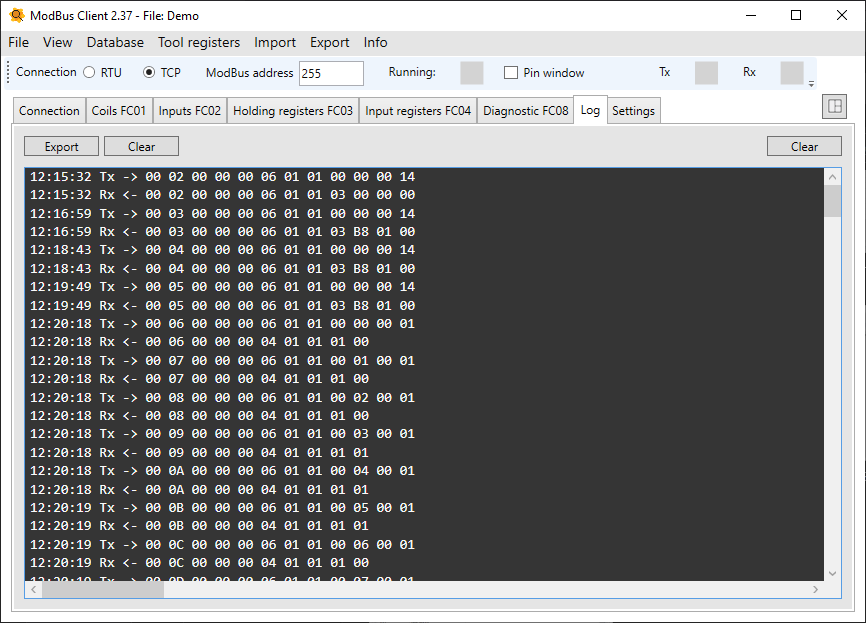
\includegraphics[width=0.70\textwidth]{../Img/ModBus_Client_Log_00.PNG}
\caption{Finestra di log}
\end{figure}

La finestra di log può anche essere aperta in una finestra separata dal menu View -> Packet Log:
(o con i tasti di scelta rapida Ctrl + L).

\begin{figure}[H]
\centering
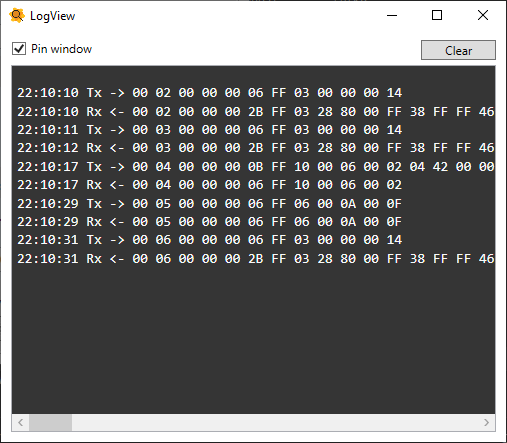
\includegraphics[width=0.35\textwidth]{../Img/ModBus_Client_Log_01.PNG}
\caption{Finestra di log ridotta}
\end{figure}

Flaggando la spunta "Pin window" la finestra rimane sempre in primo piano rispetto alle altre.

\chapter{Settings}

The settings tab contains operating parameters,
beware that the settings are tied to the profile,
changing the profile loads the respective settings.

\begin{figure}[H]
    \centering
    \includegraphics[width=0.85\textwidth]{../Img/Modbus_Client_Settings_00.PNG}
    \caption{Settings tab}
\end{figure}

\begin{itemize}
    \item \textbf{Automatically correct offset modbus addresses:}
    If checked when entering an address in the original protocol format e.g.
    holding register 40002 is automatically sent in the modbus request as address
    00001 thus eliminating the offset provided for holding registers. Otherwise it is 
    requested
    address 40002. Same for input registers (30001), discrete inputs (10001)
    or coils (00001).
    \item \textbf{Limit modbus addresses to 9998:}
    If checked, only address requests between 0 and 9998 (or corresponding address
    modbus e.g.: 10001-19999/30001-39999/40001-49999) are allowed. Otherwise, the request is sent
    whatever modbus address is entered. For example, some Beckhoff CPUs provide
    the words MW0,MW1,... starting at holding register 0x3000 (dec 12288). 
    By not checking the box
    you can then also send requests to addresses beyond the value of 9998, up to 65535.
    \item \textbf{Color cells with value > 0 / Alternating color:}
    If checked, only table rows with a value > 0 are colored, otherwise rows
    are colored alternately.
    \item \textbf{Hide user offset in tables:}
    If checked, the general offset is not displayed in the tables but is counted in the commands
    sent via ModBus. (User offset means the offset entered in the box "Offset" present
    in each tab).
    \item \textbf{Close console on startup:}
    Automatically closes the console when you start the application.
    \item \textbf{Dark mode:}
    Enable dark mode (black backgrounds, white text).
\end{itemize}

In addition to the ticks there are some parameters such as:

\begin{itemize}
    \item \textbf{Read timeout:}
    Timeout in ms for response to a command.
    \item \textbf{Loop polling interval:}
    Interval in ms between two reads for loop read commands.
\end{itemize}

For non-secure TCP connections only, it is possible to choose between two modes
of socket management:

\begin{itemize}
    \item \textbf{TCP connection mode:}
    This parameter allows you to change the TCP socket handling only for 
    non-secure mode. At the TCP socket level normally the connection is opened,
    kept open and closed at the end of its use.
    On unstable connections, however, it is more convenient to open and 
    close the socket on each request.
    The correct mode of the protocol would be the first one,
    but it often happens 
    on unstable connections (e.g., slaves connected via modem) that a connection is initiated,
    after a few reads it falls out, the socket fails and you have to reconnect again.
    With the socket going into timeout as it is no longer open on the slave 
    when the connection returns. With the second
    mode this does not happen because the socket is opened for each read 
    and closed immediately after so on a practical level this mode can come in very handy.
\end{itemize}

\chapter{Custom Templates}
\label{template}

In the "Database" -> "Open template editor" menu you can configure custom labels, bit
mappings and any integer/float/string conversions to be associated with the various registers.

\begin{figure}[H]
    \centering
    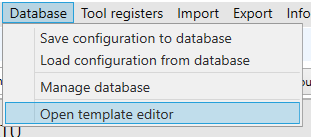
\includegraphics[width=0.4\textwidth]{../Img/Menu_Database.PNG}
    \caption{Database menu}
\end{figure}

The window for entering custom templates associated with the various registers is as follows:

\begin{figure}[H]
\centering
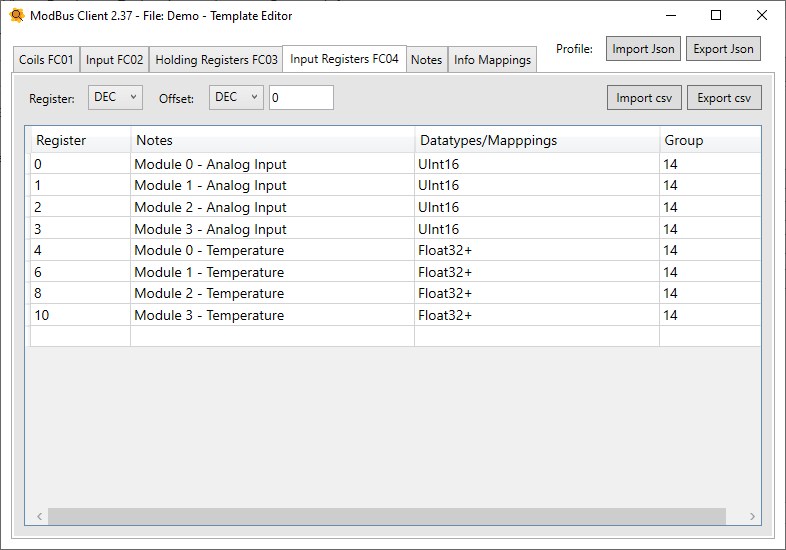
\includegraphics[width=0.80\textwidth]{../Img/ModBus_Client_Template_00.PNG}
\caption{Template editor}
\end{figure}

For each register in the template window you associate a possible label, the corresponding datatype,
and whether you want one or more resource groups to which the current group should be added.
For each register you can specify whether the value is entered in 
decimal or hexadecimal and also you can add an offset 
to the registers. In the same window you can specify whether the registers entered
are to be considered in decimal or hexadecimal and a possible offset (positive or negative)
to be added to the values entered.
For example, an offset of 100 moves the label of register 10 to the
position 110. This is convenient if, for example, a PLC has the \%MW0 starting at offset
0x4000. In this case you fill in the table starting at 0 and then simply set as the
offset the value HEX 4000.

In the case where different models of PLCs have different position
of the \%MW, to switch from one model to another is
simply change the offset without having to go and change the registers 
one by one
(negative offsets can also be applied
should it be necessary).
Following are screenshots of some examples based on the template
of the previous image:

\begin{figure}[H]
\centering
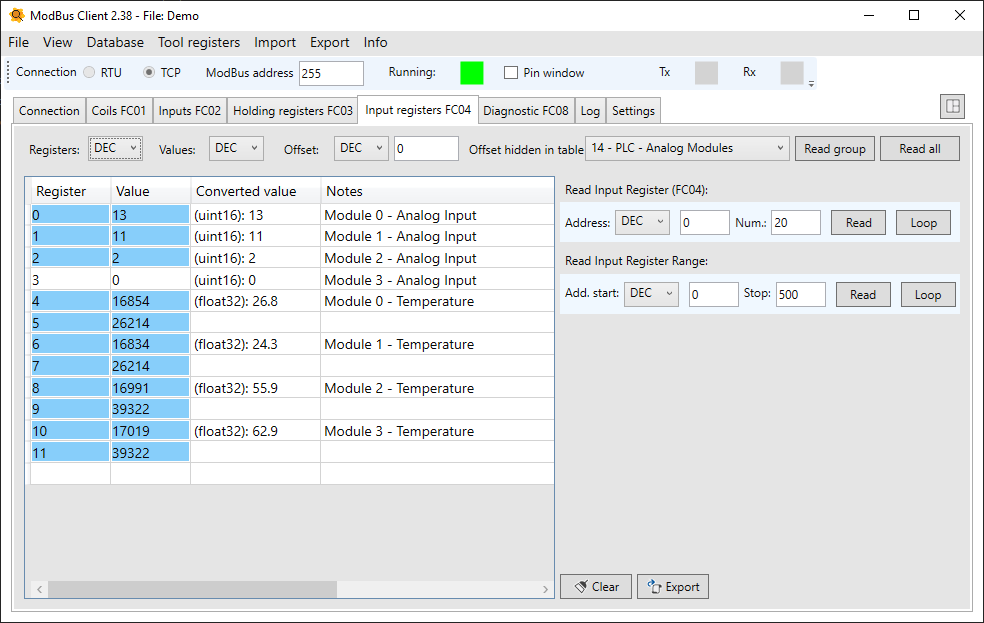
\includegraphics[width=0.70\textwidth]{../Img/ModBus_Client_Template_ReadDemo00.PNG}
\caption{Template editor}
\end{figure}

The "Notes" column displays the descriptions of the various registers 
while the "Converted Value" column displays the contents
of each register converted to the assigned datatype. In this way it is very simple to 
convert 32- or 64-bit values, floats or strings to the actual value.
By selecting a group from the drop-down menu also the client goes to read the registers
of the selected group in ascending order.

In the template window you can define multiple resource groups and
associate them with the various registers, so in the main window you can 
you can read different registers (even non-consecutive ones)
by calling up the corresponding resource group.

\begin{figure}[H]
\centering
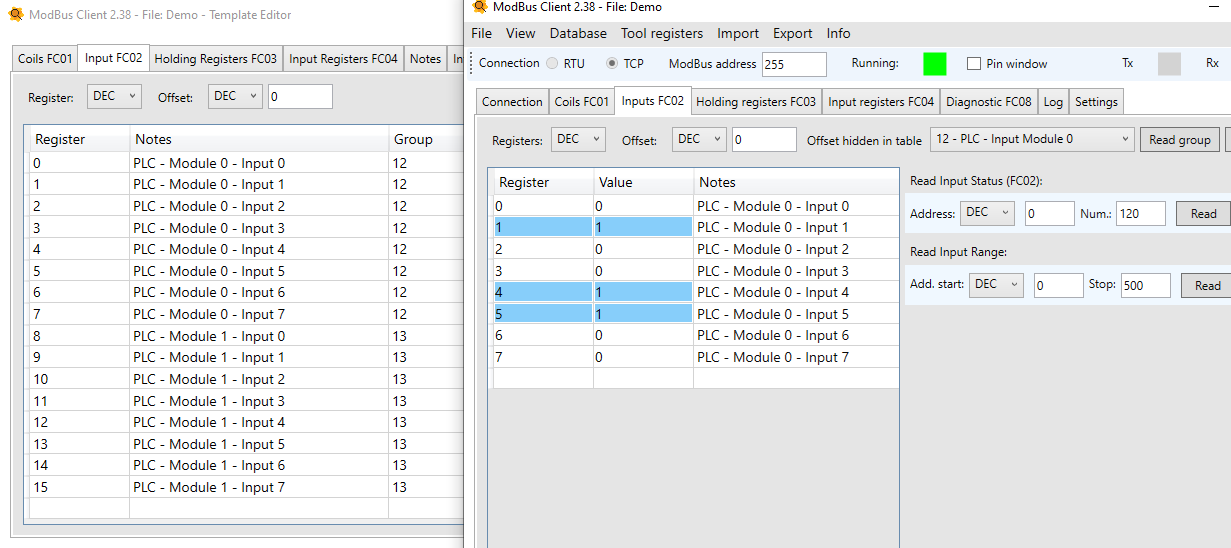
\includegraphics[width=0.85\textwidth]{../Img/ModBus_Client_Template_Group00.PNG}
\caption{Group resources}
\end{figure}

\section{Group definition}

In the "Notes" tab of the template window, it is possible to define resource groups
to be called up later in the main window. It is not necessary to enter the groups in order.

\begin{figure}[H]
\centering
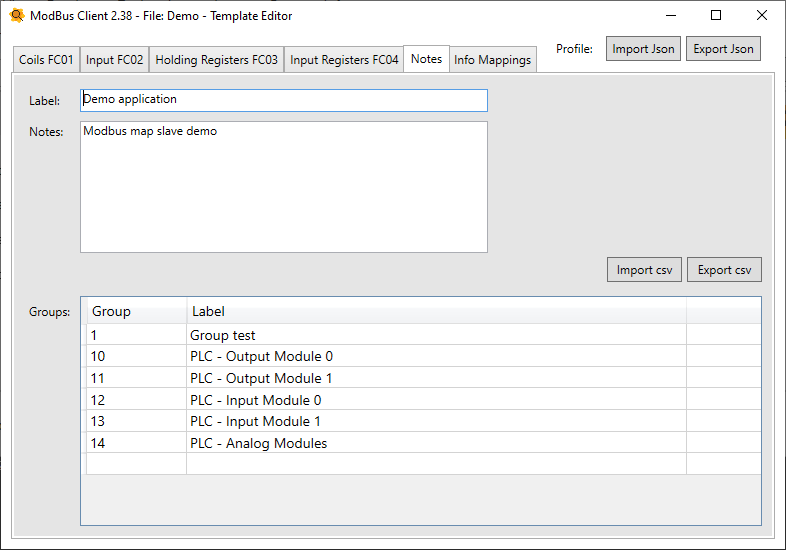
\includegraphics[width=0.70\textwidth]{../Img/ModBus_Client_Template_Group_Definition.PNG}
\caption{Group definition}
\end{figure}

The last tab "Info Mappings" contains a summary of the datatypes implemented and managed by the client.

\begin{figure}[H]
\centering
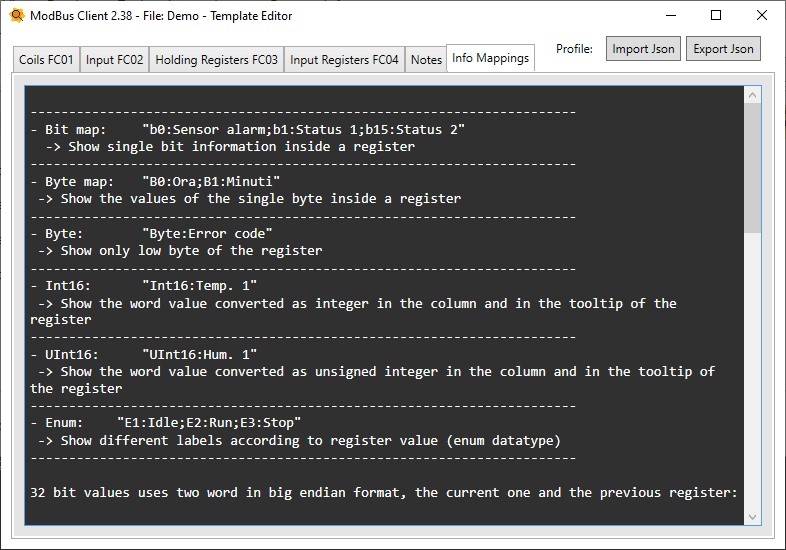
\includegraphics[width=0.70\textwidth]{../Img/ModBus_Client_Template_Info_Mappings.PNG}
\caption{Mappings info}
\end{figure}

\newpage
\section{Datatypes}

The following are the various datatypes supported by the program and configurable in a profile template.

\subsubsection{Bit map}

It shows the individual bits of the word in the line tooltip with the resource label next to it.

\begin{verbatim}
    b0:230v presence;b1:Status 1;b15:Status 2
\end{verbatim}

\subsubsection{Byte map}

It shows the two bytes of the word.

\begin{verbatim}
    B0:Hour;B1:Minutes
\end{verbatim}

\subsubsection{Int16 / UInt16}

It shows the word as a signed integer.

\begin{verbatim}
    Int16:Temp. 1
    UInt16:Counter
\end{verbatim}

The following 32-bit (two word) variables use the previous (High Word) and
current (Low Word) referenced in the Big Endian format.

\subsubsection{Float}

It collects two words and displays the data in float in the row tooltip.

\begin{verbatim}
    Float:Temperatura locale 1
\end{verbatim}

\subsubsection{Int32 / UInt32}

It collects two words and displays the data in int32 or uint32 in the line tooltip.

\begin{verbatim}
    Int32:Temperatura locale 1
    UInt32:Temperatura locale 2
\end{verbatim}

The following 64-bit variables (two words) use the three words of the previous (High Word) and
current (Low Word) referenced in the Big Endian format. With the modifiers 
format you can specify whether to use the current register and the next three.
\subsubsection{Int64 / UInt64}

\begin{verbatim}
    Int64:Timestamp start time
    UInt64:Timestamp start time
\end{verbatim}

\subsubsection{String(len[, offset])}

With string objects, it is possible to convert the contents of registers
to string (NULL terminated string). In the example below
8 bytes are converted into 8 ASCII characters with an offset of -2
(the string starts at the previous register).

\begin{verbatim}
    String(8,-2):Model
\end{verbatim}

\section{Datatype modifiers}

\subsubsection{Swap}

Adding a dash "-" or "\_swap" string multiple words
values are converted in little endian format.

\begin{verbatim}
    Swap: "UInt32-" "UInt32_swap"
\end{verbatim}

\subsubsection{Word offset}

Adding a plus sign "+" multiple words values 
uses the current register and the next ones to cast the content.

\begin{verbatim}
    Offset: "UInt32+"
\end{verbatim}

\subsubsection{Word offset + Swap}

\begin{verbatim}
    "UInt32-+" oppure "UInt32_swap+"
\end{verbatim}

Combine the previous two, use the current and next register in the Little Endian format.

\newpage

The following screenshots contains some examples
of different templates.
\\\\
Template:

\begin{figure}[H]
\centering
\includegraphics[width=0.75\textwidth]{../Img/Modbus_Client_Template_00.PNG}
\caption{}
\end{figure}

Example of final conversion:

\begin{figure}[H]
\centering
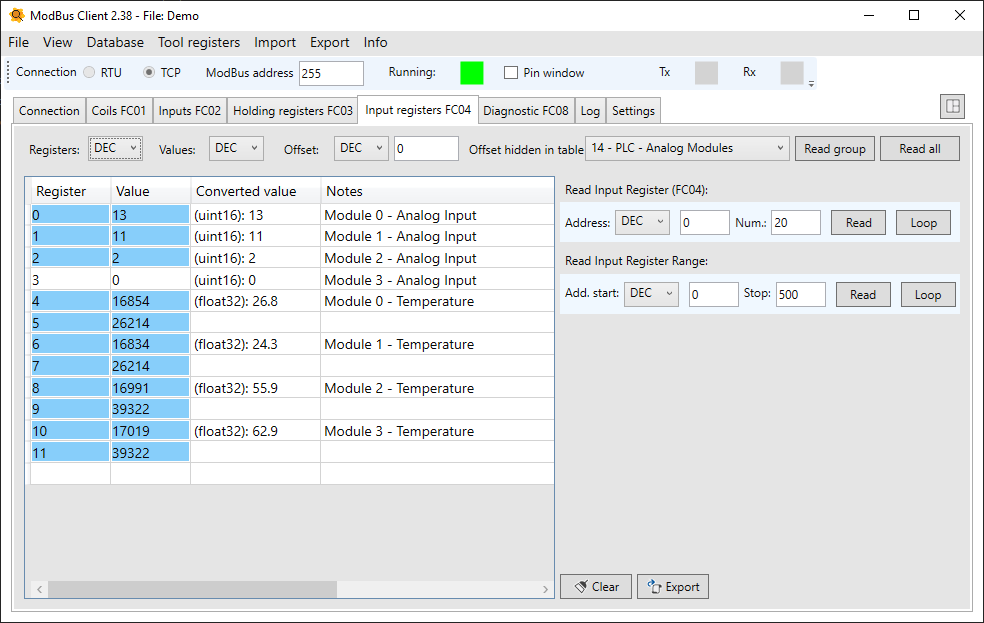
\includegraphics[width=0.75\textwidth]{../Img/ModBus_Client_Template_ReadDemo00.PNG}
\caption{}
\end{figure}

As shown in the previous image 32 bit values are casted using
two consecutive registers.

\chapter{Tools holding registers}

To edit individual bits or individual bytes/words of holding registers
there are a number of tools 
accessible from the drop-down menu
"Tool registers". The following tools apply only to holding registers, 
they are mainly used to
modify PLC objects of type \%MX,\%MB,\%MW:

\section{Bit command tool}

\begin{figure}[H]
\centering
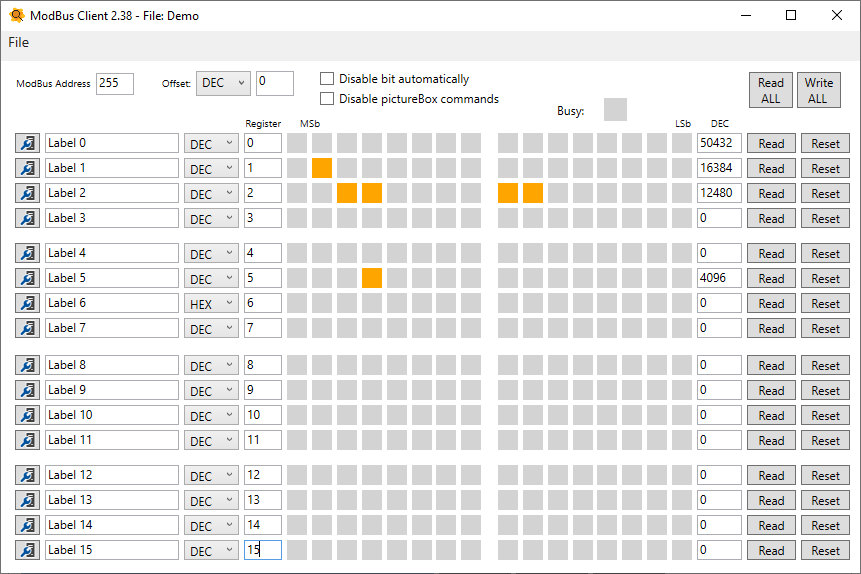
\includegraphics[width=0.85\textwidth]{../Img/Tool_Command_Bit.PNG}
\caption{Bit command tool}
\label{holding_main_win}
\end{figure}

In the Tool command bit window, you can read and view the registers in the individual bits
that make them up. By pressing on the individual bit you can reverse their state
(by default they work as a "step by step" otherwise 
if the option "disable bits automatically" is flagged on mouse click the bit is
forced to 1 and then to 0).
\newpage
Pressing the buttons next to the labels opens the window displayed in the next 
screenshot with
which you can give a specific label to the individual bit
within a word. The labels in question
refer only to the window on the previous page; they are not displayed in the tab 
"Holding registers FC 03" of the main window.

\begin{figure}[H]
\centering
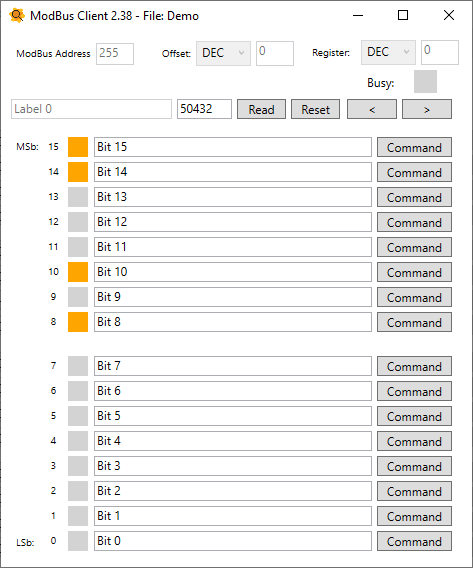
\includegraphics[width=0.55\textwidth]{../Img/Tool_Command_Bit_Label.PNG}
\caption{Bit command tool - Label Bits}
\end{figure}

The labels assigned to individual bits then become tooltips of the bits in the
main window shown in the image \ref{holding_main_win}.
The buttons "<" e ">" in the upper right-hand corner allow
to scroll between the words in the main window.

\section{Byte command tool}

\begin{figure}[H]
\centering
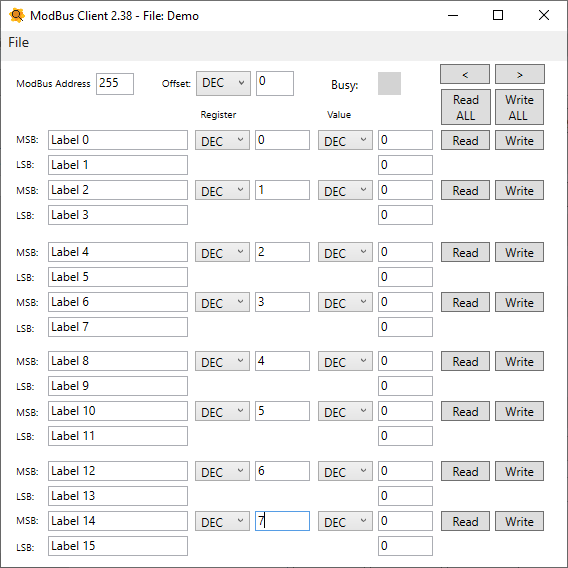
\includegraphics[width=0.55\textwidth]{../Img/Tool_Command_Byte.PNG}
\caption{Byte command tool}
\end{figure}

From the window shown above, you can send commands to individual bytes that will then be
written as word on the target. It is possible to create custom windows with which to send
commands to registers referring to different locations as well. The "<" and ">" buttons in the upper right corner allow you to
to scroll between 4 different window profiles.
Written cells are colored green while read cells are colored blue.

\section{Word command tool}

\begin{figure}[H]
\centering
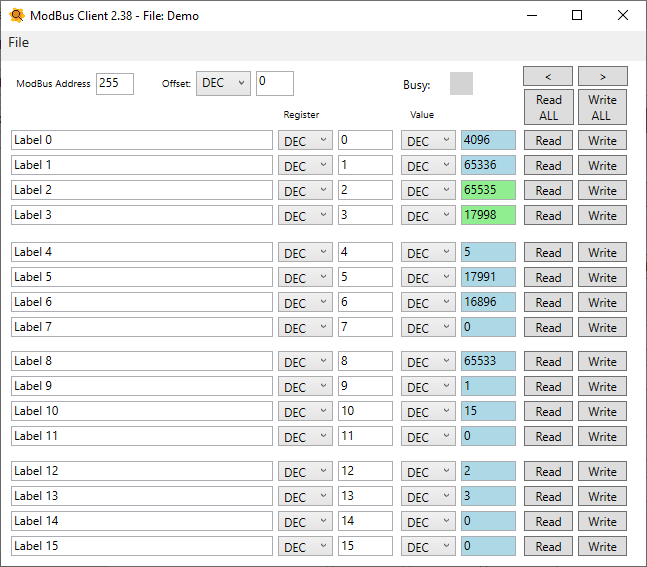
\includegraphics[width=0.55\textwidth]{../Img/Tool_Command_Word.PNG}
\caption{Word command tool}
\end{figure}

The "Word" window contains the same functions seen above for individual bytes, only
divided by word. Like the previous one with the "<" and ">" buttons in the upper right corner you can
scroll between 4 different window profiles.
Written cells are colored green while read cells are colored blue.


\chapter{Database management}

\section{Save configuration}

Pressing "Save Configuration to Database" opens a dialog box where you can enter the
name of the new custom configuration:

\begin{figure}[H]
\centering
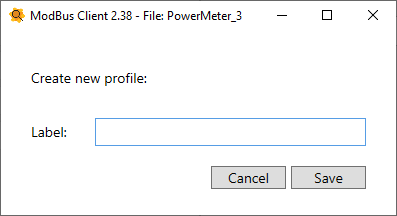
\includegraphics[width=0.35\textwidth]{../Img/SaveProfile.PNG}
\caption{Save new profile}
\end{figure}

Pressing "Save" inside the "Json" folder creates a folder with the name inserted.
DO NOT overwrite existing folders, to make changes to a custom configuration
simply open it. The changes will be saved automatically when closing
of the main window (eventually the user can save the current state from the "File"->"Save menu"
or with the shortcut "Ctrl + S").

\section{Configuration path}

The "Json" folder contains a directory for each profile. The
"Default" folder contains the program configuration when no
custom configurations is selected (if you use the program without loading a specific 
profile, any
change is saved in this folder). The other folders are generated when you save the
current configuration as a new profile.

\begin{figure}[H]
\centering
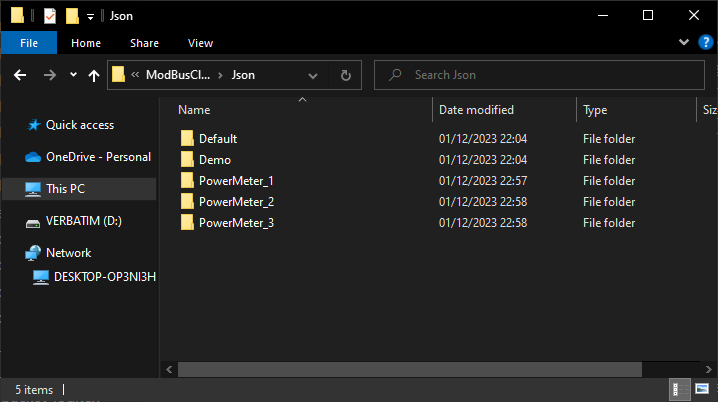
\includegraphics[width=0.45\textwidth]{../Img/DatabaseDirectory.PNG}
\caption{Database profile directory}
\end{figure}

The user in normal use does not need to make changes directly in this folder, 
simply use the forms to save and load profiles directly from the main window.

\newpage
\section{Load configuration}

Pressing "Load configuration from Database" allows you to load a configuration
previously saved:

\begin{figure}[H]
\centering
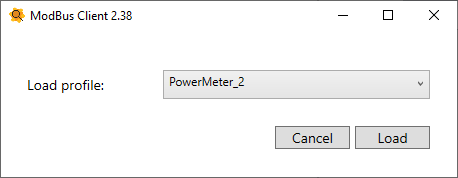
\includegraphics[width=0.45\textwidth]{../Img/LoadProfile.PNG}
\caption{Load profile}
\end{figure}

Once a custom configuration is loaded any changes entered into the program
will be saved in the custom folder without changing the structure of the configuration
"Default".

To import or export a custom Profile use the "Manage database" tool,
here you can export a profile as a .zip file, import a profile 
exported from another client or simply select the profile to be loaded.
When you close the window, automatically the selected profile is loaded into the client.

\begin{figure}[H]
\centering
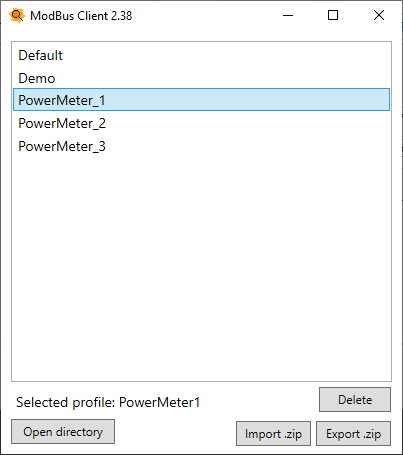
\includegraphics[width=0.40\textwidth]{../Img/DatabaseManager.PNG}
\caption{Database manager}
\end{figure}

Starting with version v2.37, profiles can be uploaded 
directly in the home tab via the drop-down menu provided:

\begin{figure}[H]
\centering
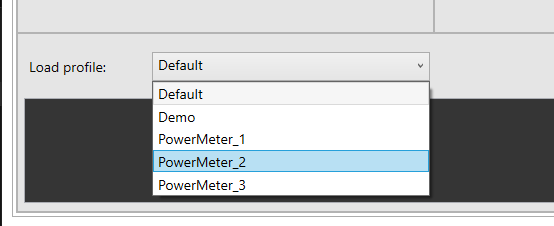
\includegraphics[width=0.50\textwidth]{../Img/ProfileHome.PNG}
\caption{Homepage profile selection}
\end{figure}

\chapter{Menu a tendina}

\section{Menu File}

Il menu file contiene i comandi per salvare la configurazione e aprire/chiudere la console.

\begin{figure}[H]
\centering
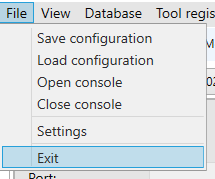
\includegraphics[width=0.3\textwidth]{../Img/Menu_File.PNG}
\caption{Menu File}
\end{figure}

\section{Menu View}

Nel menu view è possibile cambiare la lingua del programma così come visualizzare e
nascondere le colonne dei registri delle varie tab come si vede nell'immagine seguente:

\begin{figure}[H]
\centering
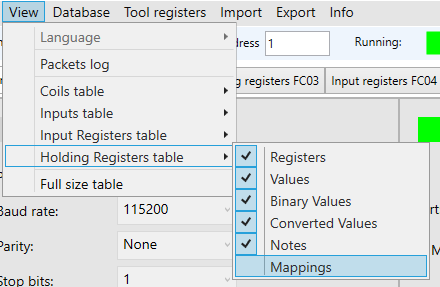
\includegraphics[width=0.6\textwidth]{../Img/Menu_View.PNG}
\caption{Menu View}
\end{figure}

\section{Menu Database}

Nel menu database è possibile creare/caricare un profilo e accedere al tool di import/export dei
profili. L'ultima voce del menu "Open temprate editor" apre la finestra di modifica dei template
personalizzati.

\begin{figure}[H]
\centering
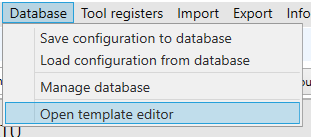
\includegraphics[width=0.45\textwidth]{../Img/Menu_Database.PNG}
\caption{Menu Database}
\end{figure}

\section{Menu Tools}

Nel menu tools è possibile aprire le finestre di comando per pilotare singoli bit/byte/word.

\begin{figure}[H]
\centering
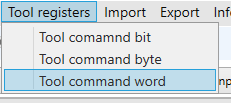
\includegraphics[width=0.32\textwidth]{../Img/Menu_Tools.PNG}
\caption{Menu Tools}
\end{figure}

\section{Menu Import}

Nel menu import è possibile inportare una tabella 
coils o holding registers esportata precedentemente
inviarla inviarla allo slave. Nel caso in cui i registri 
siano consecutivi è possibile scegliere se
inviarli singolarmente (write single coil/write single register) o in blocco 
(write multiple coils/write multiple registers).
E' possibile importare direttamente un file csv/json oppure
importare direttamente celle copiate (ctrl+c) da un foglio di calcolo
(clipboard).

\begin{figure}[H]
\centering
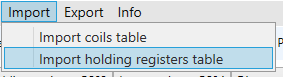
\includegraphics[width=0.4\textwidth]{../Img/Menu_Import.PNG}
\caption{Menu Import}
\end{figure}

\newpage
\section{Menu Export}

Nel menu export è possibile esportare le tabelle delle varie schede in formato csv.

\begin{figure}[H]
\centering
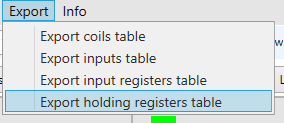
\includegraphics[width=0.4\textwidth]{../Img/Menu_Export.PNG}
\caption{Menu Export}
\end{figure}

\section{Menu Info}

Dal menu info è possibile aprire questa guida, visualizzare la licenza del programma e
data/numero di build.

\begin{figure}[H]
\centering
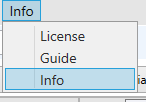
\includegraphics[width=0.25\textwidth]{../Img/Menu_Info.PNG}
\caption{Menu Info}
\end{figure}

Dal menu info si possono aprire le finestre con la versione SW 
e i contatori di pacchetti inviati e ricevuti.

\newpage

Nella finestra info è possible leggere, oltre alla versione corrente, anche data e ora di build.

\begin{figure}[H]
\centering
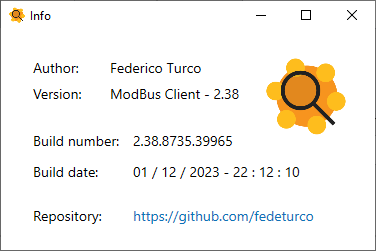
\includegraphics[width=0.5\textwidth]{../Img/Finestra_Info.PNG}
\caption{Finestra Info}
\end{figure}

La finestra statistiche mostra un riepilogo dei comandi FC inviati nella sessione corrente:

\begin{figure}[H]
\centering
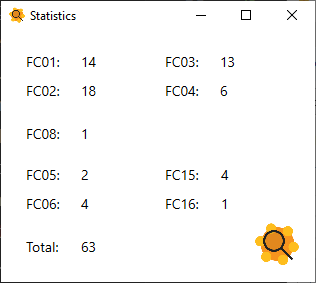
\includegraphics[width=0.5\textwidth]{../Img/Finestra_Statistiche.PNG}
\caption{Finestra Statistiche}
\end{figure}

\chapter{Shortcuts}

\begin{itemize}
\item \textbf{Ctrl + Num 1 - 9}: Select the tab with the index selected by the number pressed
\item \textbf{Ctrl + Q/Ctrl + W}: Close the window
\item \textbf{Ctrl + E}: Read the register range of the selected tab
\item \textbf{Ctrl + R}: Read the registers of the selected tab (inputs/coils/input registers/holding registers)
\item \textbf{Ctrl + T}: Open the template editing window for the currently selected profile
\item \textbf{Ctrl + Y}: Open csv/json import window
\item \textbf{Ctrl + U}: Open csv/json export window
\item \textbf{Ctrl + I}: Open software version info window
\item \textbf{Ctrl + O}: Open the menu for loading a profile
\item \textbf{Ctrl + P}: Start/Stop polling for the selected tab (loop button)
\item \textbf{Ctrl + S}: Save any changes to the currently selected profile
\item \textbf{Ctrl + Shift + S}: Open the menu to save the current profile as a new profile
\item \textbf{Ctrl + D}: Open the database management window
\item \textbf{Ctrl + F}: Enable/disable full screen mode tables
\item \textbf{Ctrl + G}: Read the group-related resources for the group selected in drop-down menu for the current tab
\item \textbf{Ctrl + H}: Read all resources entered into template for current tab
\item \textbf{Ctrl + K}: Start/Stop polling for the selected tab over the indicated range (loop button)
\item \textbf{Ctrl + L}: Open log window
\item \textbf{Ctrl + Shift + C}: Open/close client debug console
\item \textbf{Ctrl + B}: Connect/disconnect
\item \textbf{Ctrl + M}: Switch from TCP to RTU mode and vice versa
\item \textbf{Del}: Clear table contents of current tab
\end{itemize}

\chapter{Modbus Secure}
\label{secure}

The Modbus Secure protocol uses the same frames as the TCP
standard encapsulated through a TLS channel.
The TLS protocol provides an authentication system using x.509v3 certificates. 
The Modbus Secure standard requires
TLS with version 1.2 or higher (we are currently at version 1.3),
the client supports both versions (1.2 and 1.3). 
The use of certificates requires the creation of a certificate and a
private key for the server (slave), as well as for 
each client that will connect to the server (slave). 
A diagram is given below to clarify the
roles of both server-side and client-side certificates:

\begin{figure}[H]
  \centering
  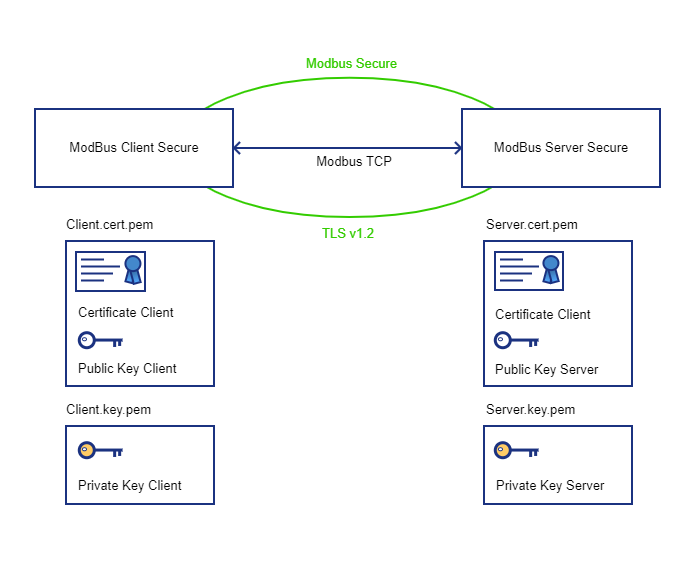
\includegraphics[width=0.8\textwidth]{../Img/schemamodbussecure.png}
  \caption{Modbus Secure certificate scheme}
\end{figure}

The standard requires certain extensions to be added to the x.509v3 certificate including an OID (Object
Identifier standardized by the International Telecomunications Union) to define the role of the client at the
time of authentication. In fact, the specification stipulates that all clients can use read functions
read functions but only clients with the role of "operator" can use write functions (of coils or holding
registers).

\newpage
\section{Modbus Secure Specification}

The main specifications of the MB-TCP\_Security-v21\_2018-07-24 regulations are given below:

\begin{itemize}
    \item The protocol version must be $\ge$ TLS 1.2
    \item Cipher suite: RSA for key exchange
    \item Cipher suite: AES128 for packet encryption
    \item Cipher suite: SHA256SUM for the integrity check of the messages
    \item Default cipher: TLS\_RSA\_WITH\_AES\_128\_CBC\_SHA256
\end{itemize}

\section{X509v3 extensions}

The following are the contents of the extensions that the standard requires 
to be added to a standard X509v3 certificate:

\begin{verbatim}
X509v3 extensions:
  X509v3 Subject Key Identifier:
      38:A4:CC:19:6D:6D:E2:AA:7C:82:75:44:A0:59:39:81:47:D3:13:F0
  X509v3 Authority Key Identifier:
      keyid:38:A4:CC:19:6D:6D:E2:AA:7C:82:75:44:A0:59:39:81:47:D3:13:F0

  X509v3 Basic Constraints:
      CA:FALSE
  X509v3 Key Usage: critical
      Digital Signature, Non Repudiation, Key Encipherment
  1.3.6.1.4.1.50316.802.1:
      ..Operator
  X509v3 Subject Alternative Name:
      IP Address:192.168.1.10
\end{verbatim}

\newpage
\section{Certificate generation}

The steps to generate certificates with openssl are as follows (multiple rows are handled so the 
commands can be copied and pasted directly to the shell console):
\\\\
Generate certificate and private key for the server (change the ip to the correct server address):

\begin{verbatim}
# Server
  openssl req -x509 -newkey rsa:4096 -sha256 -days 360 \
  -keyout server.key.pem -out server.cert.pem \
  -nodes -subj "/C=IT/ST=Italy/L=Rovereto/O=ModBusServer/OU=ModBusServer/CN=ModbusSecurityServer" \
  -addext "keyUsage=critical,digitalSignature,nonRepudiation,keyEncipherment" \
  -addext "subjectAltName=IP:192.168.1.20"
\end{verbatim}

Generate one or more certificates/private keys for the clients that 
will connect to the server (three examples are given below, 
as before the ip address must be updated with the correct one):

\begin{verbatim}
# Client 1:
  openssl req -x509 -newkey rsa:4096 -sha256 -days 360 \
  -keyout client1.key.pem -out client1.cert.pem -nodes \
  -subj "/C=IT/ST=Italy/L=Rovereto/O=ModBusClient/OU=ModBusClient/CN=ModbusSecurityClient" \
  -addext "keyUsage=critical,digitalSignature,nonRepudiation,keyEncipherment" \
  -addext "1.3.6.1.4.1.50316.802.1=ASN1:UTF8String:Operator" \
  -addext "subjectAltName=IP:192.168.1.10"
\end{verbatim}

On some operating-systems very often the certificate+private key pair is merged into a 
single password-protected file (.pfx).
To merge certificate and key into a single pfx file use the following command:

\begin{verbatim}
  openssl pkcs12 -export -out client1.pfx -inkey client1.key.pem -in client1.cert.pem
\end{verbatim}

To view the content of a certificate use the following command:

\begin{verbatim}
  openssl x509 -in client1.cert.pem -text
\end{verbatim}


\chapter{Altre note}

Il numero massimo di indirizzi che è possibile leggere con un unico comando è pari a 123 per
richieste TCP o 125 per richieste RTU. 

Se si inserisce un numero maggiore di registri viene visualizzato un messaggio di errore.

% RIFERIMENTI
%

\end{document}